\documentclass[11pt]{article}
\usepackage[a4paper,margin=0.9in]{geometry}
\usepackage{amsmath,amssymb}
\usepackage{graphicx}
\usepackage{float}
\usepackage{microtype}
\usepackage[hidelinks]{hyperref}
\emergencystretch=3em

\newcommand{\LS}{\operatorname{LS}}
\newcommand{\Proj}{\mathcal P}

\title{The Type-II Projection-Lattice Conjectures of arXiv:2006.08959\\[0.35em]
\large Fully answered by arXiv:2010.01627 and arXiv:2206.00875}
\author{Automated Mathematics Run \texttt{fa\_banach\_001}, lane 0}
\date{11 August 2026}

\begin{document}
\maketitle

\begin{center}
\fbox{\parbox{0.92\linewidth}{\textbf{Status: literature already answered.}
No new theorem is claimed.  Ayupov--Kudaybergenov settle the finite
type-\(\mathrm{II}_1\) case, and Mori settles the remaining properly infinite
type-\(\mathrm{II}_\infty\) case.  Together they prove the source's stronger
Conjecture 5.1 and consequently its weaker Conjecture 5.2.}}
\end{center}

\section{Source conjectures}

For a von Neumann algebra \(M\), let \(\LS(M)\) be its algebra of locally
measurable operators and \(\Proj(M)\) its projection lattice.  Mori's source
paper, arXiv:2006.08959, proves the desired structural theorem outside type
II and ends with the two conjectures reproduced below.

\begin{figure}[H]
  \centering
  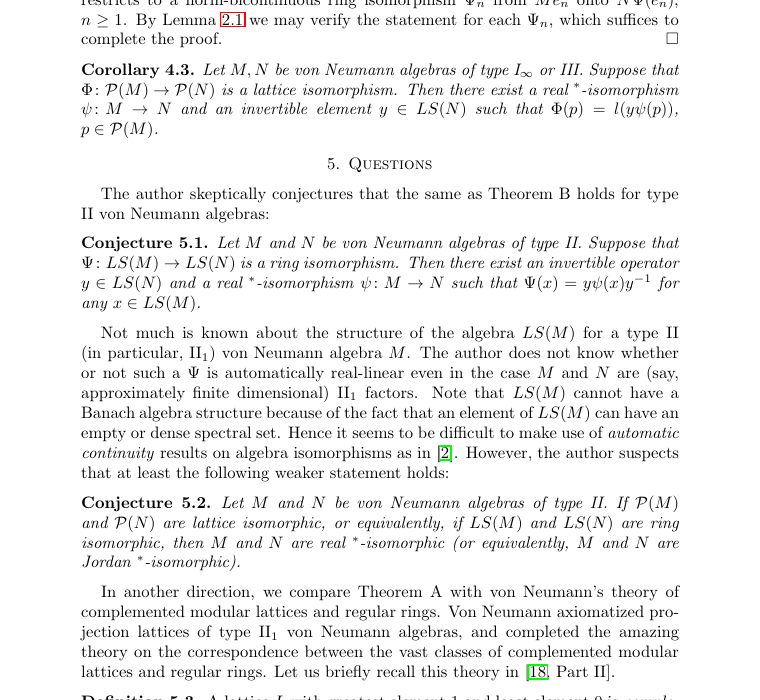
\includegraphics[width=0.80\linewidth]{figures/source_conjectures.png}
  \caption{Conjectures 5.1 and 5.2 on source PDF page 19
  (printed page 9) of arXiv:2006.08959v1.}
\end{figure}

The stronger statement is:
\[
\begin{gathered}
 M,N\text{ of type II},\quad
 \Psi:\LS(M)\longrightarrow\LS(N)\text{ a ring isomorphism}\\
 \Longrightarrow\quad
 \Psi(x)=y\psi(x)y^{-1},
\end{gathered}
\]
where \(y\in\LS(N)\) is invertible and
\(\psi:M\to N\) is a real \(^{*}\)-isomorphism extending to the locally
measurable algebras.  Conjecture 5.2 asks only whether a lattice isomorphism
\(\Proj(M)\cong\Proj(N)\) forces \(M,N\) to be real \(^{*}\)-isomorphic,
equivalently Jordan \(^{*}\)-isomorphic.

\section{The finite type-\texorpdfstring{\(\mathrm{II}_1\)}{II1} answer}

Ayupov and Kudaybergenov, arXiv:2010.01627, explicitly say that their main
result confirms Conjecture 5.1 of the source.  Their Theorem 1.4 states that
for type-\(\mathrm{II}_1\) algebras \(M,N\), every ring isomorphism
\(\Phi:S(M)\to S(N)\) has the form
\[
 \Phi(x)=a\Psi(x)a^{-1}
\]
for an invertible \(a\in S(N)\) and a real \(^{*}\)-isomorphism
\(\Psi:M\to N\) extending to \(S(M)\to S(N)\).  Since a finite von Neumann
algebra satisfies \(\LS(M)=S(M)\), this is exactly the
type-\(\mathrm{II}_1\) part of Conjecture 5.1.  Corollary 1.5 gives the
projection-lattice equivalence requested in Conjecture 5.2.

\begin{figure}[H]
  \centering
  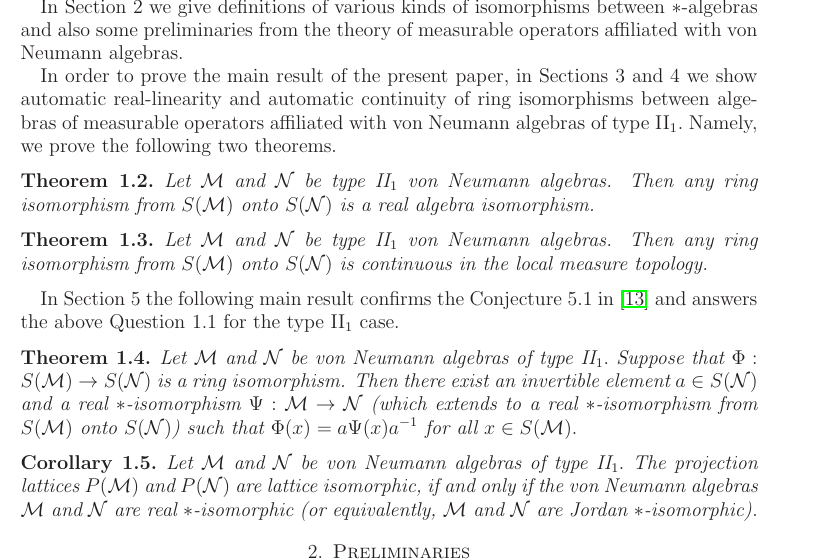
\includegraphics[width=0.88\linewidth]{figures/type_ii1_answer.png}
  \caption{Theorems 1.2--1.4 and Corollary 1.5 on PDF page 2 of
  arXiv:2010.01627v2.}
\end{figure}

\section{The type-\texorpdfstring{\(\mathrm{II}_\infty\)}{II-infinity} answer}

Mori's later paper arXiv:2206.00875 identifies
\(\mathrm{II}_\infty\) as the last blank case.  Theorem 1.2 proves that if
\(M,N\) are of type \(\mathrm{II}_\infty\), every ring isomorphism
\(\Psi:\LS(M)\to\LS(N)\) is
\[
 \Psi(x)=y\psi(x)y^{-1}
\]
with \(y\in\LS(N)\) invertible and \(\psi:M\to N\) a real
\(^{*}\)-isomorphism extending to \(\LS(M)\to\LS(N)\).

\begin{figure}[H]
  \centering
  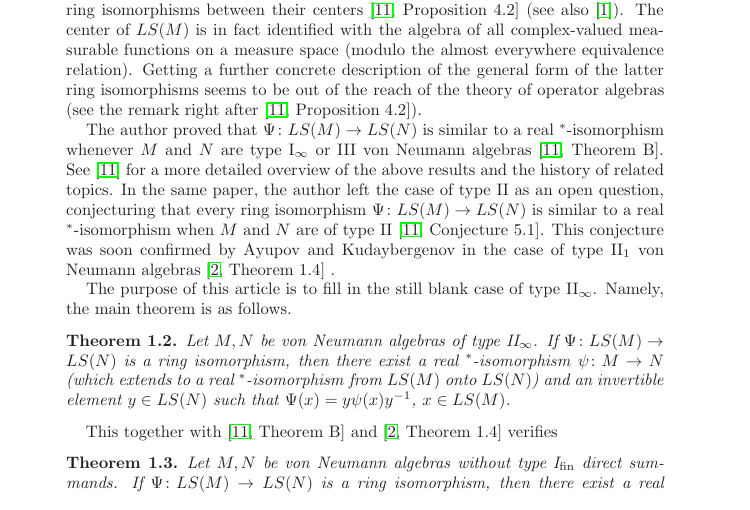
\includegraphics[width=0.68\linewidth]{figures/type_ii_infinity_answer.png}
  \caption{Theorem 1.2 and the combined theorem on PDF page 2 of
  arXiv:2206.00875v2.}
\end{figure}

The same page explicitly combines this theorem with
Ayupov--Kudaybergenov's Theorem 1.4 and the source's Theorem B.  Its Theorem
1.3 gives the inner-twisted real-\(^{*}\) form for all von Neumann algebras
without finite type-I direct summands, and Theorem 1.4 gives the corresponding
classification of projection-lattice isomorphisms.  In particular both
source conjectures hold for every type-II algebra, including arbitrary
central mixtures of finite and properly infinite type-II summands.

\section{Conclusion and verification}

The later results match the source quantifiers and conclusion exactly:

\begin{center}
\begin{tabular}{lll}
\hline
Source scope & Later theorem & Status\\
\hline
type \(\mathrm{II}_1\) & arXiv:2010.01627, Thm.\ 1.4 & answered\\
type \(\mathrm{II}_\infty\) & arXiv:2206.00875, Thm.\ 1.2 & answered\\
all type II & arXiv:2206.00875, Thms.\ 1.3--1.4 & answered\\
\hline
\end{tabular}
\end{center}

The source and both supporting PDFs were downloaded from arXiv.  The
displayed source passage and theorem statements were checked directly
against those PDFs, not inferred from abstracts alone.  A bounded search of
the run indexes found no prior packet for arXiv:2006.08959.  The source
conjectures therefore require no new proof attempt and are classified
\texttt{literature\_already\_answered}.

\begin{thebibliography}{9}
\bibitem{Mori2020}
M.~Mori,
\emph{Lattice isomorphisms between projection lattices of von Neumann algebras},
Forum Math. Sigma 8 (2020), e49; arXiv:2006.08959.

\bibitem{AK2021}
Sh.~A. Ayupov and K.~K. Kudaybergenov,
\emph{Ring isomorphisms of Murray--von Neumann algebras},
J. Funct. Anal. 280 (2021), 108891; arXiv:2010.01627.

\bibitem{Mori2023}
M.~Mori,
\emph{Ring isomorphisms of type \(\mathrm{II}_\infty\) locally measurable
operator algebras},
Bull. Lond. Math. Soc. 55 (2023), 2525--2538; arXiv:2206.00875.
\end{thebibliography}

\end{document}
